\documentclass[tikz,border=2mm]{standalone}
\usepackage{tikz}
\usepackage{tikz-feynman}
\tikzfeynmanset{compat=1.1.0}

\begin{document}

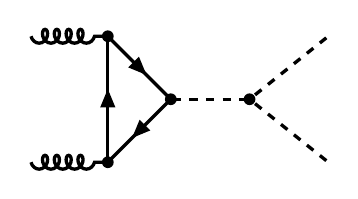
\begin{tikzpicture}
\begin{feynman}
    % Vertici principali
    \vertex [inner sep=0pt](i1) at (0,0.8) {};
    \vertex [inner sep=0pt](i2) at (0,-0.8) {};
    \vertex [inner sep=0pt](v1) at (1,0.8) {};
    \vertex [inner sep=0pt](v2) at (1,-0.8) {};
    \vertex [inner sep=0pt](v3) at (1.8,0) {};
    \vertex [inner sep=0pt](v4) at (2.8,0) {};
    \vertex [inner sep=0pt](f1) at (3.8,0.8) {};
    \vertex [inner sep=0pt](f2) at (3.8,-0.8) {};

    % Marker visibili
    \node[circle, fill=black, inner sep=1.5pt] at (v1) {};
    \node[circle, fill=black, inner sep=1.5pt] at (v2) {};
    \node[circle, fill=black, inner sep=1.5pt] at (v3) {};
    \node[circle, fill=black, inner sep=1.5pt] at (v4) {};
    % Diagramma
    \diagram* {
        (i1) -- [gluon,line width=1.2pt] (v1),
        (i2) -- [gluon,line width=1.2pt] (v2),
        (v2) -- [fermion,line width=1.2pt] (v1),
        (v1) -- [fermion,line width=1.2pt] (v3),
        (v3) -- [fermion,line width=1.2pt] (v2),
        (v3) -- [dashed,line width=1.2pt] (v4),
        (f2) -- [dashed,line width=1.2pt] (v4),
        (f1) -- [dashed,line width=1.2pt] (v4),
    };
\end{feynman}
\end{tikzpicture}


\end{document}

% pdflatex feynman_diag.tex

% pdftoppm -png -r 300 gluon_fusion_1.pdf gluon_fusion_1